\chapter{Estado del arte}

En este capítulo, se va a comentar el estado actual de la inteligencia artificial relacionada con el póker, así como la relación de la inteligencia artificial con los juegos de mesa.


\section{Relación histórica de la inteligencia artificial con los juegos de mesa.}

El estudio del póker es algo que se lleva haciendo en los últimos años, en diversos ámbitos de investigación, no únicamente en la inteligenica artificial, como la teoría de juegos incluso en algunos estudios de economia. \cite{Billings} 

En el ámbito de la inteligencia artificial, los juegos se han utilizado como puntos de referencia, ya que sirven como una forma de evaluar los resultados usando dichos juegos como pruebas de campo.
 Uno de los ejemplos de este tipo de resultados es Deep Blue\cite{deepblue1}, una supercomputadora desarrollada por IBM para jugar ajedrez, que se enfrentó a Garry Kasparov\footnote{Garry Kasparov fue un jugador de ajedrez profesional que se convirtió en el campeón mundial de ajedrez en 1985, título que mantuvo hasta el año 2000 (de manera indisputable hasta 1993, fecha en la que se produjo la división de títulos por las disputas entre la Federación internacional de Ajedrez, FIDE, y la Asociación profesional de Ajedrez, PCA). Desde 1993 hasta 2000 se matuvo como campeón mundial de Ajedrez clásico. En junio del año 2000, perdió el título de campeón mundial de ajedrez ante Vladimir Krammik. } dos veces. Ambos enfrentamientos se realizaron al mejor de 6 partidas. 

El primero de estos enfrentamientos tuvo lugar en 1996, con un resultado de 4-2 en favor de Kasparov (3 victorias para el campeón mundial, 2 empates y 1 victoria para Deep Blue). A pesar de la derrota de Deep Blue, este enfrentamiento supuso un hito histórico, ya que fue la primera vez que un campeón mundial perdió una partida clásica de ajedrez siguiendo las reglas de torneos frente a una máquina.

La revancha de este enfrentamiento se produjo en 1997, en la cual una versión mejorada de Deep Blue se volvió a enfrentar a Kasparov. Sin embargo, en este enfrentamiento se produjo la victoria de Deep blue con un resultado de 3.5-2.5 (2 victorias de Deep blue, una victoria de Kasparov y 3 empates). Esta victoria significó que, por primera vez en la historia, un programa informático de ajedrez ganaba al campeón mundial, marcando un antes y un después en la historia de la inteligencia artificial.\cite{deepblue1}

Deep blue supuso una gran inspiración para el desarrollo de la inteligencia artificial, que supuso un nuevo campo de investigación, usando tanto el ajedrez como otros juegos. 

Uno de los juegos donde también se logró es el juego de las damas. En 2007 Jonathan Schaeffer publicó un artículo en el que explicaba cómo había resuelto el problema de las Damas con el software Chinook, en el cual mostraba los resultados que habían obtenido él y su equipo durante el desarrollo de Chinook. \cite{chinook}

Incluso se consiguió en el Go\footnote{Juego de estrategia de origen chino de dos jugadores, en el que los jugadores, por turnos, van colocando fichas idénticas de su color en los cruces de las líneas que conforman el tablero (lo habitual es un tablero de 19x19 líneas, dando lugar a 361 posibles posiciones) hasta que ambos jugadores deciden pasar de forma consecutiva, momento en el cual la partida acaba y se determina el ganador haciendo un conteo de los puntos.}, considerado como uno de los juegos clásicos más desafiantes de cara a la inteligencia artificial, ya que la cantidad de posicionamientos dentro del tablero, los diferentes posibles movimientos en cada uno de los posibles tableros y el arbol de decisiones es mucho más complejo que en el ajedrez (la complejidad del arbol de decisiones del Go es del orden de $10^{360}$ mientras que la del ajedrez es del orden de $10^{123}$). \cite{gametree} 

Esto se logró en 2017, donde David Silver y su equipo lograron desarrollar un software capaz de ganar a otros softwares de Go y ganó al ganador Europeo de Go en un 5-0, siendo el primero en derrotar a un jugador profesional de Go en un enfrentamiento de torneo.\cite{Go}

El factor común que tienen estos tres juegos y que les separa de juegos como el póker, es que todos estos juegos son juegos de información perfecta, en el que todos los jugadores conocen toda la información de la partida en cada momento, mientras que en los juegos de información imperfecta hay elementos que se desconocen para los jugadores. Se tratará en más profundidad la gestión de la información en los juegos en el apartado \ref{sec:info}.



\section{Inteligencia artificial en el póker.}

La gestión de información imperfecta (en la que se desconoce parte de la información) es el tipo de gestión de información que genera más interés desde el punto de vista de la inteligencia artificial, ya que es la que se puede utilizar para modelar situaciones de la vida real (tales como pruebas de seguridad, acuerdos comerciales, subastas o estrategias de negocio). Esto implica que las estrategias a la hora de desarrollar inteligencia artificial cambien completamente respecto a los juegos de información perfecta.\cite{libratusScience2}

Entre estos juegos de información imperfecta, uno de los más usados para hacer estudios de teoría de juegos e inteligencia artificial es el póker. Además de tener que cambiar las estrategias a la hora de desarrollar la inteligencia artificial, hay que ser capaz de gestionar las acciones para mantener, en la medida de lo posible, esa información privada de los demás jugadores y es necesario considerar todos los factores de una partida de póker en conjunto de cara a la hora de plantear una estrategia (tales como versatilidad, las apuestas, las acciones, cuando ver o no una apuesta, todos los aspectos matemáticos del póker...), es decir, que no pueden considerarse por separado. Todo estos factores hacen del póker un desafío para la inteligencia artificial, lo cual hace más interesante su estudio para este ámbito.\cite{libratusScience2}

Al haber tantas posibles variables a la hora de desarrollar inteligencia artificial en el ámbito del póker, los desarrolladores de inteligencia artificial han tenido que recurrir a la herramienta de la abstracción para intentar reducir, en la medida de lo posible, esas variables. 

La abstracción consiste en aplicar restricciones a los espacios de estrategia de los jugadores, ya sea mediante una abstracción de información o una abstracción de acciones.
La abstracción de información consiste en agrupar información, creando un "bloque" de información y trabajar en torno a ese bloque de información. Por otro lado, la abstracción de acciiones limita alguna de las acciones que los jugadores pudiera hacer en una partida real, incluyendo la posibilidad de eliminar algunas de estas posibles acciones. \cite{abstraction}

Cada uno de los programadores de inteligencia artificial desarrolla estas limitaciones de una manera distinta, lo que afecta a cómo se plantea su software. Se van a tratar dos softwares distintos: \textit{Poki} y \textit{Libratus}.

\subsection{\textit{Poki}}

\textit{Poki} \cite{Billings} es un software diseñado por el departamento de Ciencias de Computación de la universidad de Alberta. \textit{Poki} simula partidas de varios jugadores, durante la cual modela cada uno de los oponentes en función de sus acciones, analiza todos los aspectos del juego (la fuerza de la mano, el potencial de la misma, lar ronda en la que se encuentra, las apuestas...) y, en conjunto con el modelado de cada oponente, establece las acciones posibles para tomar en esa mano y decide que acción tomar.

\begin{figure}[h]
\centering
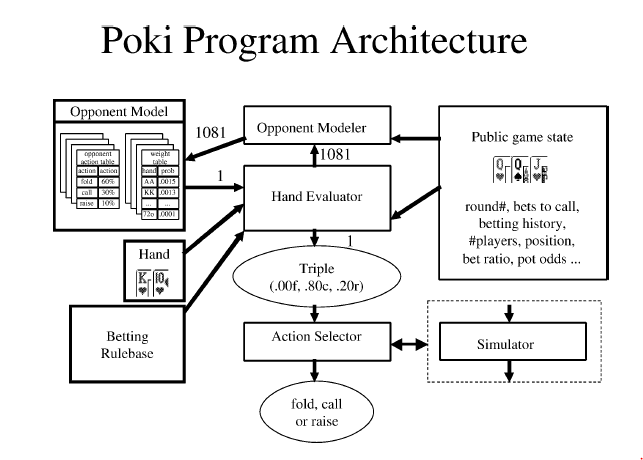
\includegraphics[width=0.9\textwidth]{figuras/Poki.png}   
\caption{Arquitectura de Poki \cite{Billings}}
\label{fig:poki}
\end{figure}

En el preflop, \textit{Poki} modela a cada oponente como una distribución de probabilidades según la mano que puedan tener, modelado que se genera con una estrategia de apuestas basadas en reglas y obtiene parámetros de cada uno de los oponentes en función de las acciones de cada jugador. Tras el flop, \textit{Poki} evalua el valor de la mano en el contexto de la ronda (considerando cada uno de los oponentes y su modelado, así como las apuestas y las cartas, entre otros factores), usando una  apuesta basadas en reglas más complejas que en el preflop y generando las posibles acciones que pueda tener el programa en ese contexto, además de utilizar un simulador que itera este proceso teniendo en cuenta diferentes posibles manos de los oponentes. Este proceso cíclico se repite cada vez que sea necesario actuar por parte de \textit{Poki}.

La abstracción en este software se centra en el procesado de datos, pues las acciones las procesa usando una probabilidad triple. Esto se refiere a que cada modelado, incluido el del propio \textit{Poki}, se basa en un conjunto ordenado de tres valores: PT = \{f,c,r\}. Cada uno de estos valores representa la distribución de probabilidades de que la próxima acción de ese jugador sea pasar, ver o subir la apuesta, respectivamente.\cite{Billings}

Esta abstracción permite gran parte de los elementos problemáticos de una partida de póker (tales como la fuerza o el potencial de una mano) en un único elemento (siendo una abstracción de información). 

Si bien este software ha ido mejorando con el paso del tiempo, pudiendo vencer a jugadores de cada vez mayor nivel, este software no es capaz de enfrentarse adecuadamente a un jugador profesional. Por otro lado, es uno de los pocos softwares que simulan partidas de múltiples jugadores (ya que una de las abstracciones más habituales que hacen los programas de póker es centrarse en la modalidad heads-up, o modalidad de dos jugadores, ya que elimina tanto el modelado de múltiples oponentes cómo el factor de la posición con respecto al dealer, que en una partida real tiene una importancia relevante).

\subsection{\textit{Libratus}}

\textit{Libratus} \cite{libratusScience2, libratusScience} es un software de inteligencia artificial diseñado para jugar partidas de Póker sin límite de apuestas de dos jugadores (Heads-Up No-Limit poker o HUNL poker) desarrollado por Noam Brown and Tuomas Sandholm, miembros del departamento de Ciencias de Computación de la universidad Carnagie Mellon
Cómo se ha mencionado al final del apartado anterior, el optar por esta modalidad elimina la complejidad computacional de múltiples oponentes y el posicionamiento. Además de eso, también evita escenarios donde las malas decisiones de uno de los jugadores convierta a un jugador en ganador, aunque la estrategia de dicho jugador no sea tan buena como la de otros.

El funcionamiento de \textit{Libratus} consiste en tres módulos de funcionamiento:
\begin{enumerate}
\item  \textbf{Módulo de Plano de estrategias.} Este módulo genera una abstracción del estado de juego, llamada plano de estrategias, mucho más pequeña y simple de resolver en la que se incluyen estrategias basadas en teoría de juegos que sirven de guía a la hora de jugar las rondas: siendo bastante detalladas para las primeras rondas y una aproximación para las rondas posteriores.
\item \textbf{Módulo de Solución de Subjuegos anidados.} Una vez que se alcanzan rondas mas avanzadas de la partida, este módulo genera una nueva abstracción más pequeña y precisa dentro de la primera abstracción y la resuelve en tiempo real, considerando esta solución siempre como parte de la estrategia incluida en el plano de estrategias para la partida entera. Si se da el caso de que el oponente realice una acción que no se contempla en esta segunda abstracción, se resuelve un subjuego que si incluye esa acción. A esto es lo que denominan resolución de subjuegos anidados.
\item \textbf{Módulo de Mejora.} Este módulo sirve para mejorar el plano de estrategias, pues completa los subjuegos faltantes de la abstracción del plano de estrategias, computando estrategias para cada uno de estos subjuegos faltantes. Además de eso, y a modo de optimización, prioriza unos u otros subjuegos en función de las acciones del oponente, ya que el intentar computar cada uno de los subjuegos restantes generaría un arbol tan grande para que esto pueda llegar a ser completado sin perder optimización del programa.
\end{enumerate}

\begin{figure}[h]
\centering
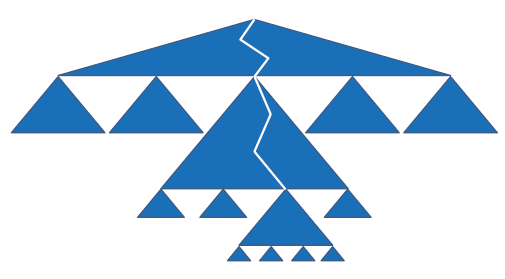
\includegraphics[width=0.9\textwidth]{figuras/Libratus.png}   
\caption{Visualización del funcionamiento de la abstracción de Libratus \cite{libratusScience2} y de la resolución de subjuegos anidados. Partiendo del plano de estrategias (triangulo superior), se generan varias abstracciones con sus propias estrategias (los triángulos en la base del plano de estrategias), siendo el triangulo más grande la que corresponde a la abstracción precisa generada analizando las acciónes (el camino blanco) que el oponente ha ido tomando, lo cual genera otros subjuegos anidados.}
\label{fig:libratus}
\end{figure}

Este software se probó tanto contra otros softwares de HUNL poker, entre ellosBaby Tartarian8\footnote{El Bot Baby Tartarian8 es un bot de inteligencia artificial para póker desarrollado también por Noam Brown y Tuomas Sandholm, que había derrotado al resto de inteligencias artificiales participantes en la Competición Anual de Poker por Ordenador (Annual Computer Poker Competition o ACPC) en el año anterior al desarrollo de Libratus con un margen de 12 ± 10 y 24 ±20 mili-ciega grande (mbb) por partida a los softwares más fuertes de dicho ACPC.} , así como algunos de mejores profesionales de HUNL Poker, resultando ganador \textit{Libratus} en ambos casos. \cite{libratusScience2, libratusScience}

